\documentclass{standalone}
\usepackage{pgfplots}
\pgfplotsset{compat=1.13}
\usepackage{amsmath}
\colorlet{paleBlue}{blue!10!white}



\begin{document}

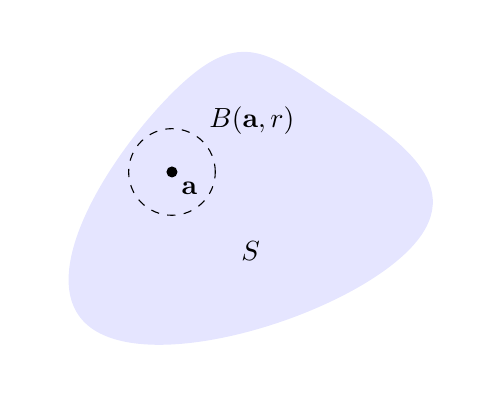
\begin{tikzpicture}
    \fill[paleBlue] plot [smooth cycle, tension=1] coordinates {(0,0) (1,3) (3,3) (4,1)};
    \draw[dashed] (1,2) circle (.55) node[above right=10pt]{\(B(\mathbf{a},r)\)};
    \fill[black] (1,2) circle (2pt) node[anchor=north west]{\(\mathbf{a}\)};
    \node at (2,1){\(S\)};
\end{tikzpicture}

\end{document}